\documentclass[journal]{IEEEtran}
\usepackage[T1]{fontenc}
\usepackage{amsmath,amsfonts,amssymb}
\usepackage{array,booktabs,cite,graphicx,url,xcolor,microtype}
\usepackage[scaled=0.88]{newtxtt}
\graphicspath{{figures/}}
\newcommand{\pp}{\,\mathrm{pp}}
\newtheorem{definition}{Definition}

\usepackage{xr-hyper}
\externaldocument[supp-]{supplement}[supplement.pdf]
\setcounter{dbltopnumber}{3}
\renewcommand{\dbltopfraction}{0.90}
\renewcommand{\textfraction}{0.08}
\usepackage[colorlinks=true,citecolor=blue,linkcolor=blue,urlcolor=blue,breaklinks=true]{hyperref}
\begin{document}

\title{Cross-Track Sentinel-1 Land-Cover Classification with Two-Acquisition Interferometric Coherence}

\author{Shiji~Fan,
        Daniel~Albuquerque,~\IEEEmembership{Member,~IEEE},
        Pedro~Pinho,~\IEEEmembership{Senior Member,~IEEE},
        and~Ming~Shen,~\IEEEmembership{Senior Member,~IEEE}%
\thanks{This work is funded by national funds through FCT--Funda\c{c}\~ao para a
Ci\^encia e a Tecnologia, I.P., and, when eligible, co-funded by EU funds under
project/support UID/50008/2025--Instituto de Telecomunica\c{c}\~oes, with DOI
identifier \protect\url{https://doi.org/10.54499/UID/50008/2025}.}%
\thanks{S. Fan, D. Albuquerque, and P. Pinho are with the University of Aveiro,
Aveiro, Portugal, and Instituto de Telecomunica\c{c}\~oes, Portugal (e-mail:
shiji.fan@ua.pt; dfa@ua.pt; ptpinho@ua.pt). M. Shen is with Aalborg University,
Aalborg, Denmark (e-mail: mish@es.aau.dk). Corresponding author: Shiji Fan.}%
}

\markboth{Manuscript submitted to IEEE Transactions on Geoscience and Remote Sensing}%
{Fan \MakeLowercase{\textit{et al.}}: Two-Acquisition Coherence for Cross-Track Classification}

\maketitle

\begin{abstract}
Interferometric coherence records temporal scattering stability that complements SAR backscatter intensity. Its contribution to cross-track land-cover classification at a two-acquisition budget is the focus of this study. We evaluate four Sentinel-1 tracks over the eastern Netherlands, spanning ascending and descending passes and $12.2^\circ$ in incidence angle. A single 12-day coherence measurement augments a 28-dimensional intensity representation derived from the same image pair. Spatial model selection and evaluation use a 400\,m training exclusion, with three sampling seeds and twelve directed cross-track transfers. Coherence increases five-class balanced accuracy by $6.30\pp$ (95\% confidence interval: $5.25$--$8.19$) for random forest and $6.99\pp$ ($5.78$--$9.39$) for a support vector classifier. The corresponding overall-accuracy gains are $1.95\pp$ and $1.64\pp$. Class-level analysis locates the largest improvement in built-up land: its misclassification as forest falls from $17.5\%$ to $0.8\%$ for random forest. Spring-trained models retain balanced-accuracy gains of $5.03\pp$ and $5.23\pp$ on autumn acquisitions. Additional spatial and nonlinear coherence transformations provide no improvement over the raw scalar. These results identify repeat-pass coherence as a compact source of complementary class information for land-cover mapping across orbital tracks with limited acquisitions.
\end{abstract}

\begin{IEEEkeywords}
Synthetic aperture radar (SAR), Sentinel-1, interferometric coherence, cross-track transfer, land-cover classification, observation budget, spatial cross-validation.
\end{IEEEkeywords}

\section{Introduction}
\label{sec:related}
\IEEEPARstart{S}{atellite} synthetic aperture radar (SAR) supports land-cover monitoring through cloud cover and without daylight. Sentinel-1 observations provide complementary measurements of surface backscatter and interferometric coherence for this task~\cite{Jacob2020,Sica2019}. Using several orbital tracks expands the available observation schedule, but also changes how the radar illuminates the surface. Incidence angle, look direction, and terrain affect the measured backscatter; radiometric terrain correction addresses the associated variation in illuminated area~\cite{Small2011}. A classifier deployed across tracks must therefore use features that retain class information as the observation configuration changes. This requirement becomes particularly important when only a short sequence of acquisitions is available.

Repeat-pass interferometric coherence measures the magnitude of the normalized complex correlation between coregistered SAR acquisitions~\cite{Bamler1998,Touzi1999}. It adds sensitivity to changes in the scattering configuration over the interval between observations. Stable structures can retain correlation, whereas changes within vegetation reduce it. This contrast provides information complementary to backscatter power and has been used for forest mapping and the separation of forests from artificial surfaces~\cite{Sica2019,Zhuang2024,Aghababaei2026}. The two observables thus describe different aspects of the same scene: intensity records scattering strength, while coherence records the persistence of the complex return. Their combination offers a physical basis for improving class separation with a small number of acquisitions.

Much of the evidence for this complementarity comes from time-series classification. Jacob \textit{et al.}~\cite{Jacob2020} compared coherence-based representations across land-cover classifiers, while Mestre-Quereda \textit{et al.}~\cite{MestreQuereda2020} combined backscatter and coherence from a full year of Sentinel-1 observations for crop-type mapping. Recent studies connect interferometric observables to crop growth and use coherence time series to detect seeding dates~\cite{Yuan2024,ChenX2025}. Their value depends on when observations sample the vegetation cycle: L\"ow \textit{et al.}~\cite{Low2024} examined crop-specific signatures across years and orbits, directly connecting these observables to phenology.

Recent SAR classifiers exploit temporal structure with distribution-aware prototypes~\cite{Guo2025}, polarimetric feature sequences~\cite{LiuN2025}, and learned spatial--temporal representations~\cite{Russo2025,He2025}. Multisensor attention models combine these sequences with optical observations~\cite{Anandakrishnan2025}, while optical spatial--temporal fusion and parcel-based pipelines extend crop mapping to larger regions~\cite{Li2026,Sanchez2026}. Multifrequency experiments further show how polarimetric and interferometric measurements complement one another~\cite{Romero2026}. These approaches extract information along additional observation dimensions. The acquisition budget is therefore an essential part of any comparison of representation quality.

Scattering-based representations offer another route to class separation. Recent work uses dual-polarization target descriptors for Sentinel-1 clustering~\cite{Verma2025} and scattering powers for single-date crop classification with simulated NISAR data~\cite{Nihar2026}. Statistical approaches characterize class separability through intensity distributions~\cite{Negri2025} or geodesic polarimetric parameters~\cite{daSilva2026}. Multipass covariance modeling explicitly exploits temporal correlations when classifying scattering symmetries~\cite{Hanis2025}. Particularly relevant here, Zhuang \textit{et al.}~\cite{Zhuang2024} use repeat-pass coherence to distinguish vegetation volume scattering from rotated built-up structures. These results motivate testing temporal stability as a compact additional observable in dual-polarization land-cover mapping.

The accompanying intensity sequence also affects the measured benefit of coherence. In the 18-scene crop-mapping experiment of Zhao \textit{et al.}~\cite{Zhao2024}, dual-polarization backscatter achieved 95.12\% overall accuracy (OA), and adding VV coherence increased OA to 95.33\%. The resulting $0.21\pp$ increment describes the additional information available after a growing-season intensity sequence. A two-acquisition budget presents a different inference problem. It supplies one coherence measurement and two intensity observations, with no seasonal trajectory to learn. Moreover, those two intensity images still support spatial texture, polarization ratios, and gradients. Quantifying coherence's marginal value therefore requires a comparison against features extracted from the same image pair, including a developed intensity representation.

Cross-track deployment adds a second dimension to that comparison. Geographic transfer experiments have documented the dependence of crop-classification performance on the training and deployment regions~\cite{Orynbaikyzy2022}. Multisource domain generalization and frequency-based style mixing address distribution changes in remote-sensing image classification and segmentation~\cite{Han2024,Iizuka2024}; meta-learning also supports transfer between polarimetric SAR datasets and frequency bands~\cite{Luo2025}. These studies motivate separating the information supplied by an observable from the adaptation supplied by a learning algorithm. Here, observations from four tracks cover the same study area, allowing directional transfers across orbital configurations on common geographic support. Each track supplies its own repeat-pass pair for coherence estimation; the classifier is then transferred between tracks. Evaluating the corresponding in-track predictions gives a direct interpretation of the coherence increment. Gains in both settings indicate additional class discrimination, while a change in the difference between in-track and cross-track accuracy measures its effect on the transfer penalty.

This study quantifies the marginal classification value of a single 12-day coherence measurement under a fixed two-acquisition Sentinel-1 budget (Fig.~\ref{fig:workflow}). Four tracks yield twelve directional transfers, evaluated with random forest and support-vector classifiers. A five-representation design compares basic intensity features, a 28-dimensional intensity representation, and the addition of raw or spatially transformed coherence. All comparisons share the acquisition pairs and training budgets, with a 400\,m training-to-validation exclusion during spatial model selection. Five-class balanced accuracy measures the average class-level benefit, and paired spatial block bootstrap contrasts quantify its uncertainty. Combining these contrasts with in-track evaluation and class-level confusion analysis identifies where coherence contributes information and how that contribution affects cross-track deployment.

\begin{figure*}[!t]
\centering
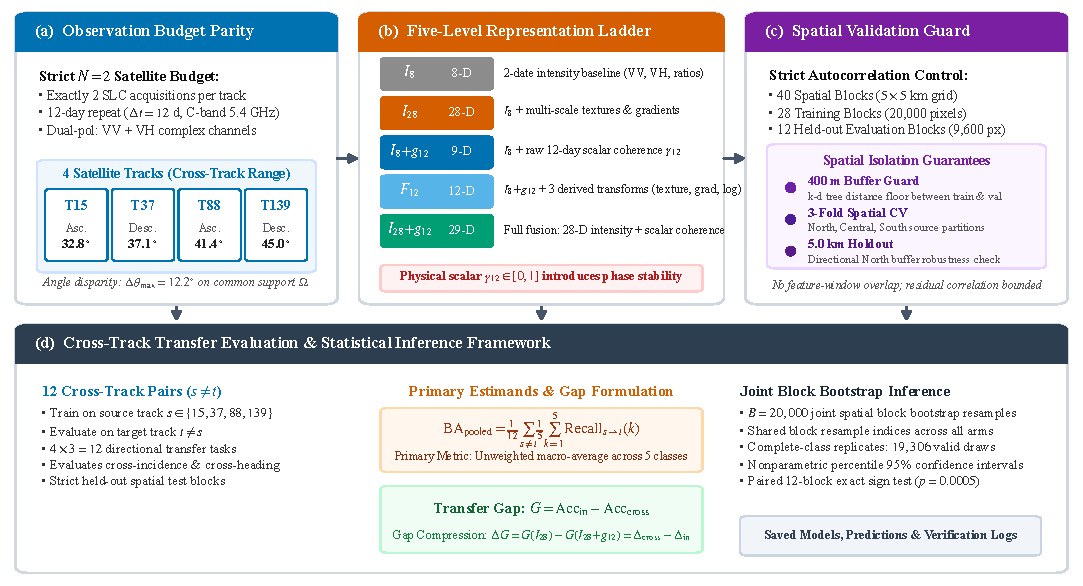
\includegraphics[width=0.98\textwidth]{fig1_workflow.pdf}
\caption{Evaluation of coherence under a two-acquisition budget. (a) Shared SLC pairs for each track. (b) Five representations comparing intensity texture, raw coherence, and derived coherence features. (c) Spatial model selection with a 400\,m training-to-validation exclusion and additional 5\,km directional holdouts. (d) Classification and transfer contrasts with paired block resampling across compared representations.}
\label{fig:workflow}
\end{figure*}


\section{Data and Acquisition Geometry}
\subsection{Study Area and Orbital Tracks}
The study covers a $43.08\times38.60$\,km region in the eastern Netherlands, bounded by $[6.00^\circ\mathrm{E},51.98^\circ\mathrm{N},6.54^\circ\mathrm{E},52.38^\circ\mathrm{N}]$. Its landscape includes grassland, cropland, forest, settlements, and inland water. All layers use UTM Zone 32N (EPSG:32632) on a $1077\times965$ grid with 40\,m spacing.

Four Sentinel-1A IW tracks provide 12-day repeat-pass pairs from May 2024 (Table~\ref{tab:dataset}). T15 and T88 are ascending; T37 and T139 are descending. Mean incidence angles on the common support range from $32.798^\circ$ to $45.003^\circ$. The four tracks define twelve directed cross-track transfers and four in-track evaluations on the same geographic support.

\subsection{SAR Processing}
\label{sec:chain}
Products were generated from Sentinel-1A IW SLC acquisitions through ASF HyP3~\cite{HyP3}, using GAMMA for interferometric processing and radiometric terrain correction. The four interferometric pairs share 10 range by 2 azimuth looks and a 40\,m UTM posting. Processing used Goldstein--Werner filtering with $\alpha=0.6$, minimum-cost-flow unwrapping, and the Copernicus GLO-30 DEM~\cite{CopernicusDEM}. The classification feature is the magnitude of normalized complex correlation, $g_{12}$, from the repeat-pass pair~\cite{Touzi1999}.

Radiometric terrain correction produces terrain-flattened $\gamma^0$ backscatter~\cite{Small2011} at 10\,m. T15 and T37 products are delivered in dB; T88 and T139 products are converted from linear power to dB at native resolution. All four tracks then undergo bilinear interpolation to the 40\,m analysis grid. Supplementary Section S-IV records this processing convention.

Spatial feature windows extend to $7\times7$ pixels for intensity and $3\times3$ pixels for coherence. The 400\,m exclusion used in model selection and evaluation exceeds the extent of overlapping feature windows. Within-class coherence autocorrelation decreases from $0.72$--$0.74$ at 40\,m to $0.11$--$0.15$ at 400\,m, and falls below $0.08$ at 5\,km.

\subsection{Reference Labels and Common Support}
\label{sec:ground_truth}
ESA WorldCover 2021 v200~\cite{ESAWorldCover2021} and CORINE Land Cover 2018~\cite{CORINE2018} provide reference labels. Categorical labels are aligned by nearest-neighbor resampling and harmonized as forest, grassland, cropland, built-up, and water. The existing WorldCover preprocessing applies a one-column alignment correction before extraction on the analysis grid.

The four-track sensor-valid mask $M_2$ contains 633,308 pixels, with finite intensity and valid coherence and incidence-angle values on every track. Intersecting $M_2$ with the minimum-mapping-unit mask gives $\Omega=608,825$ pixels. Of these, $U_2=600,317$ have valid labels in both reference products, and $C_2=287,013$ have matching labels. The primary models use $C_2$ for training and evaluation. Label-sensitivity experiments also use $U_2$ and individual reference products. The two-acquisition sensor mask matches the recorded four-baseline mask, $M_2=M_4$.

\begin{figure*}[!t]
\centering
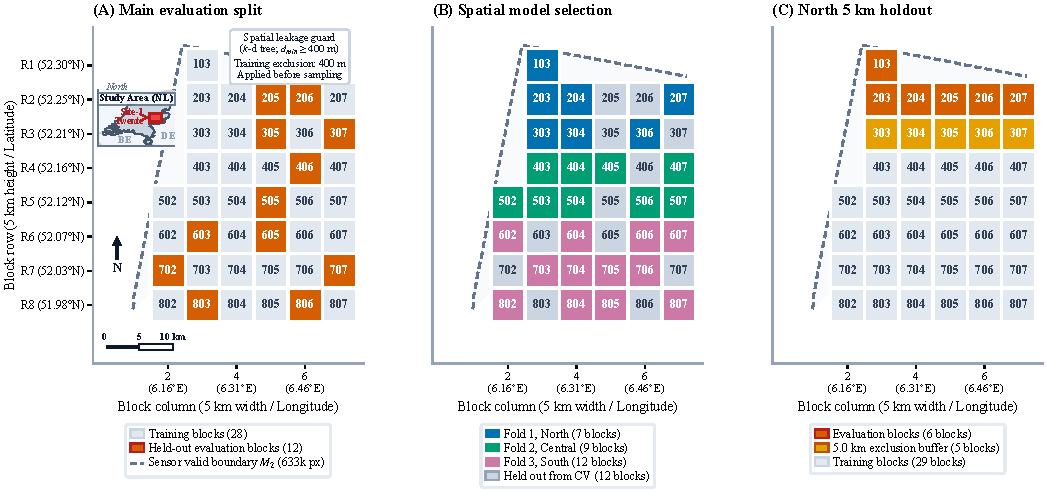
\includegraphics[width=0.92\textwidth]{fig2_study_area.pdf}
\caption{Spatial partitions on the common four-track footprint. (A) The primary split uses 28 training blocks and 12 evaluation blocks. (B) Source-track model selection uses three spatial folds within the training blocks. A 400\,m exclusion separates training candidates from validation or evaluation pixels. (C) A directional holdout with a 5\,km excluded block row; directional results are reported in Section~\ref{sec:label_independence}.}
\label{fig:study_area}
\end{figure*}

\begin{table*}[!t]
\caption{Observation Geometry, Acquisition Parameters, and Pixel Support Summary for the Four-Track Sentinel-1 Dataset}
\label{tab:dataset}
\centering
\scriptsize
\setlength{\tabcolsep}{4pt}
\begin{tabular}{lccrrcccr}
\toprule
Track & Pass & IW & Abs.\ orbit & $\theta_{\text{AOI}}$ & $\theta_{\Omega}$ & Reference acq.\ ($t_1$) & Repeat acq.\ ($t_2$) & $B_\perp$ (m) \\
\midrule
T15  & Ascending  & IW1 & 53812 & $32.502^\circ$ & $\mathbf{32.798^\circ}$ & 2024-05-10 17:17:24 & 2024-05-22 17:17:23 & $+198.20$ \\
T37  & Descending & IW2 & 53834 & $37.482^\circ$ & $\mathbf{37.125^\circ}$ & 2024-05-12 05:50:38 & 2024-05-24 05:50:38 & $+156.34$ \\
T88  & Ascending  & IW2 & 53885 & $41.132^\circ$ & $\mathbf{41.387^\circ}$ & 2024-05-15 17:25:29 & 2024-05-27 17:25:29 & $-72.19$ \\
T139 & Descending & IW3 & 53761 & $45.003^\circ$ & $\mathbf{45.003^\circ}$ & 2024-05-07 05:42:28 & 2024-05-19 05:42:28 & $-21.41$ \\
\bottomrule
\end{tabular}
\\[3pt]
\parbox{\textwidth}{\footnotesize Acquisition parameters are from the delivered HyP3 metadata. $\theta_{\rm AOI}$ and $\theta_\Omega$ denote mean ellipsoid incidence angles over the full grid and the common analysis support, respectively. The latter defines the $12.205^\circ$ angular span used throughout. Ascending and descending headings are $-15.6^\circ$ and $195.3^\circ$.}
\end{table*}

The four-track image subset in Fig.~\ref{fig:multitrack_sar_coherence} shows the same settlements and agricultural parcels under different viewing configurations. Backscatter brightness and texture vary across tracks, while built surfaces retain higher coherence than the surrounding vegetation.

\begin{figure*}[!t]
\centering
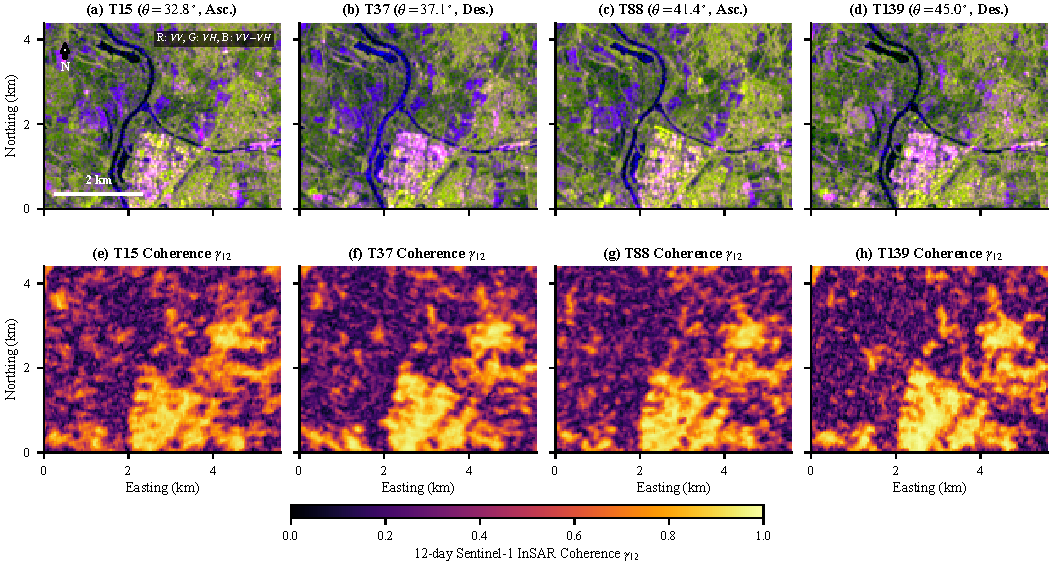
\includegraphics[width=0.98\textwidth]{fig3_multitrack_sar_coherence.pdf}
\caption{Sentinel-1 observations over a $4.4\times5.6$\,km subset around Goor and the Twentekanaal. Top row: dual-polarization backscatter composites for T15, T37, T88, and T139. Bottom row: the corresponding 12-day coherence fields. Built surfaces have high coherence against lower-coherence agricultural and forest cover.}
\label{fig:multitrack_sar_coherence}
\end{figure*}


\section{Methodology}
\subsection{Feature Representations}
\label{sec:ladder}
Five representations share an eight-feature intensity base. Their paired contrasts measure the added value of intensity texture, raw coherence, and coherence transformations.
\begin{enumerate}
    \item \textbf{$I_8$ (8-D Base Intensity)}: Dual-date backscatter temporal means $\overline{VV} = (VV_1 + VV_2)/2$, $\overline{VH} = (VH_1 + VH_2)/2$, cross-ratio $\overline{RT} = \overline{VH} - \overline{VV}$, temporal differentials $\Delta VV = VV_2 - VV_1$, $\Delta VH = VH_2 - VH_1$, $\Delta RT$, and $3 \times 3$ local standard deviations $\sigma_{3\times 3}(\overline{VV})$, $\sigma_{3\times 3}(\overline{VH})$.
    \item \textbf{$I_{28}$ (28-D Full Intensity Baseline)}: $I_8$ augmented with absolute temporal differences $|\Delta VV|, |\Delta VH|, |\Delta RT|$, temporal channel extrema ($\min, \max$), multi-scale spatial textures ($5 \times 5, 7 \times 7$ local standard deviations), and Sobel gradient magnitudes of $\overline{VV}$, $\overline{VH}$, and $\overline{RT}$, $3\times3$ standard deviations of $\Delta VV$ and $\overline{RT}$, and the four original date--polarization channels.
    \item \textbf{$I_8+g_{12}$ (9-D Raw Coherence Augmentation)}: $I_8$ augmented with the single 12-day interferometric coherence scalar $g_{12} = \gamma_{12}$.
    \item \textbf{$F_{12}$ (12-D Derived Coherence Representation)}: $I_8+g_{12}$ augmented with spatial coherence texture $\sigma_{3\times 3}(g_{12})$, coherence gradient magnitude $\|\nabla g_{12}\|$, and non-linear log-transform $\ln(1 - g_{12} + 10^{-4})$.
    \item \textbf{$I_{28}+g_{12}$ (29-D Competitive Augmented Baseline)}: The full 28-D intensity baseline augmented with the identical raw coherence scalar $g_{12}$.
\end{enumerate}
Spatial filters use the four-track sensor-valid mask, independently of the reference labels. Standard deviations use normalized masked filters; gradients use sensor-valid neighborhoods. The feature set contains intensity and coherence magnitude.

\subsection{Spatial Model Selection and Evaluation}
\label{sec:partition}
The scene is partitioned into 40 usable $5\times5$\,km blocks. The primary split assigns 28 blocks to training and twelve to evaluation (Fig.~\ref{fig:study_area}). Sampling 800 consensus pixels per evaluation block gives 9,600 test pixels per target track. Within the training blocks, three spatial folds cover the northern, central, and southern portions.

For each fold, a $k$-d tree contains all validation candidates. Training candidates within 400\,m of any validation candidate are removed before sampling. The same exclusion is applied around the main evaluation pool. It removes $1.3$--$2.2\%$ of fold training candidates and 16,040 of 164,743 main training candidates. Minimum realized distances are 417.6, 400.0, and 400.0\,m for the folds, and 400.0\,m for the final training samples.

Model selection maximizes mean three-fold balanced accuracy separately for each learner, representation, and source track. RF~\cite{Breiman2001} uses 300 trees, with $\mathrm{max\_features}\in\{\sqrt{D},0.5D,D\}$ and minimum leaf sizes in $\{1,5\}$. SVC~\cite{Cortes1995} uses an RBF kernel, $C\in\{0.1,1,10,100\}$, and $\gamma\in\{0.1,1,10\}\gamma_{\rm scale}$. Its robust scaler is fitted within the source training fold. Ties within $0.1\pp$ use the recorded simpler-parameter ordering. Model selection comprises 1,080 fold fits across 40 configurations.

Selected parameters are frozen for final training on 20,000 pixels per source track and representation, sampled without replacement using seeds 17, 29, and 43. These configurations produce 120 fitted models. Each model predicts all four target tracks. Supplementary Section S-I lists the selected parameters.

\subsection{Metrics and Paired Inference}
For each seed, cross-track balanced accuracy averages class recall within each transfer and then averages the twelve directed transfers:
\begin{equation}
\mathrm{BA}_{\rm cross}=\frac{1}{12}\sum_{s\ne t}\frac{1}{5}\sum_{k=0}^{4}\frac{C_{s\to t}(k,k)}{\sum_{j=0}^{4}C_{s\to t}(k,j)}.
\end{equation}
Here $C_{s\to t}$ pools the evaluation blocks for a source--target pair. Reported performance is the mean across three sampling seeds, with seed standard deviations shown separately. Overall accuracy (OA) is the fraction of correctly classified evaluation pixels. The transfer gap is
\begin{equation}
G=\mathrm{Accuracy}_{\rm in}-\mathrm{Accuracy}_{\rm cross}.
\end{equation}
Coherence increments compare the augmented and intensity-only representations on identical observations. Gap reduction equals $\Delta_{\rm cross}-\Delta_{\rm in}$.

The spring analysis draws twelve evaluation blocks with replacement in each of 20,000 bootstrap iterations. Compared representations, track pairs, and seeds share the same draw. Five-class BA intervals use the 19,306 draws containing every class; the other 694 omit water. The main point estimates use the full sample. Repeated predictions of a pixel remain grouped within its spatial block during resampling.

Temporal evaluation applies the 48 frozen spring models for $I_{28}$ and $I_{28}+g_{12}$ to October 2024 observations of the same tracks. Autumn BA intervals use the bias-corrected and accelerated block bootstrap. All 20,000 draws are retained, with BA averaged over the classes present in both arms in the 633 draws with class dropout. Autumn OA uses percentile intervals. These conventions and the separate label-sensitivity protocol are documented in Supplementary Sections S-II and S-III.

\section{Empirical Results}

\subsection{Primary Performance and Representation Ablation}
\label{sec:primary}
\label{sec:ablation}
Adding $g_{12}$ to the 28-D intensity baseline increases cross-track balanced accuracy from $67.03\%$ to $73.33\%$ for RF and from $66.72\%$ to $73.71\%$ for SVC (Table~\ref{tab:benchmark}; Fig.~\ref{fig:primary_contrasts}). The paired increments are $+6.30\pp$ $[5.25,8.19]$ and $+6.99\pp$ $[5.78,9.39]$. Overall accuracy increases by $+1.95\pp$ $[1.32,2.65]$ and $+1.64\pp$ $[0.91,2.47]$. Intervals use 20{,}000 joint block bootstrap draws; the five-class analysis retains 19{,}306 draws containing all classes. Open water occurs in three evaluation blocks and is absent from the remaining draws.

The representation ladder separates the contributions of intensity texture and coherence (Fig.~\ref{fig:coherence_ablation}). Expanding $I_8$ to $I_{28}$ adds $+2.66\pp$ $[1.97,3.34]$ for RF and $+2.73\pp$ $[1.96,3.66]$ for SVC. Adding raw coherence directly to $I_8$ yields $+8.60\pp$ $[7.24,10.36]$ and $+10.10\pp$ $[8.14,12.44]$. The twenty added intensity features therefore supply $31\%$ and $27\%$ of the increments obtained from the single coherence scalar. The compact $I_8{+}g_{12}$ representation reaches $72.97\%$ and $74.09\%$ balanced accuracy, respectively, compared with $73.33\%$ and $73.71\%$ for $I_{28}{+}g_{12}$.

The three derived transformations provide no additional gain. Adding $\sigma_{3\times3}(g_{12})$, $\|\nabla g_{12}\|$, and $\ln(1-g_{12}+10^{-4})$ to $I_8{+}g_{12}$ produces $F_{12}$, whose paired increment is $-0.28\pp$ $[-0.65,-0.08]$ for RF and $-0.20\pp$ $[-0.38,+0.07]$ for SVC. Raw coherence supplies the measured benefit of the interferometric representation.

\begin{figure*}[!t]
\centering
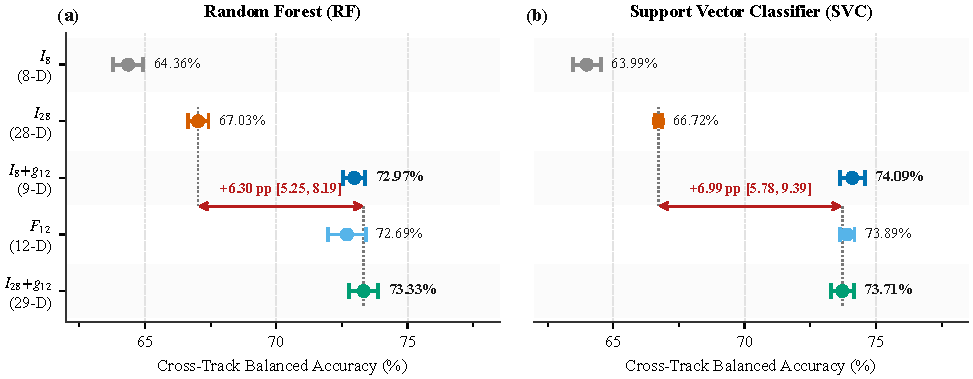
\includegraphics[width=0.98\textwidth]{fig4_primary_contrasts.pdf}
\caption{Cross-track balanced accuracy for five representations: (a) RF and (b) SVC. Markers give full-sample estimates; error bars show one standard deviation across three training-sample seeds. Arrows mark the paired coherence increment over $I_{28}$, with 95\% spatial block-bootstrap intervals.}
\label{fig:primary_contrasts}
\end{figure*}

\begin{table*}[!t]
\caption{Cross-track performance (mean $\pm$ seed standard deviation) and in-track minus cross-track gap $G$. The representations use the same two acquisitions and 400\,m spatial exclusion.}
\label{tab:benchmark}
\centering
\scriptsize
\setlength{\tabcolsep}{3pt}
\begin{tabular}{llcccc}
\toprule
Learner & Repr. & Cross-Track OA (\%) & Cross-Track BA (\%) & $G_{\text{OA}}$ (pp) & $G_{\text{BA}}$ (pp) \\
\midrule
RF & $I_8$ (8-D) & 67.83\,$\pm$\,0.12 & 64.36\,$\pm$\,0.58 & 3.81 & 4.70 \\
RF & $I_{28}$ (28-D) & 69.42\,$\pm$\,0.08 & 67.03\,$\pm$\,0.40 & 3.62 & 4.76 \\
RF & $I_8{+}g_{12}$ (9-D) & 70.29\,$\pm$\,0.08 & 72.97\,$\pm$\,0.42 & 3.48 & 4.35 \\
RF & $F_{12}$ (12-D) & 70.66\,$\pm$\,0.13 & 72.69\,$\pm$\,0.72 & 3.42 & 4.47 \\
RF & $I_{28}{+}g_{12}$ (29-D) & \textbf{71.37}\,$\pm$\,0.06 & \textbf{73.33}\,$\pm$\,0.55 & 3.35 & 4.12 \\
\midrule
SVC & $I_8$ (8-D) & 70.30\,$\pm$\,0.09 & 63.99\,$\pm$\,0.52 & 3.06 & 4.91 \\
SVC & $I_{28}$ (28-D) & 71.13\,$\pm$\,0.05 & 66.72\,$\pm$\,0.14 & 3.31 & 4.74 \\
SVC & $I_8{+}g_{12}$ (9-D) & 72.24\,$\pm$\,0.06 & \textbf{74.09}\,$\pm$\,0.48 & 2.78 & 3.86 \\
SVC & $F_{12}$ (12-D) & 72.23\,$\pm$\,0.03 & 73.89\,$\pm$\,0.28 & 2.83 & 3.89 \\
SVC & $I_{28}{+}g_{12}$ (29-D) & \textbf{72.78}\,$\pm$\,0.03 & 73.71\,$\pm$\,0.43 & 3.12 & 4.44 \\
\bottomrule
\end{tabular}
\\[3pt]
\parbox{\textwidth}{\footnotesize \textbf{Incremental coherence gain} ($I_{28}+g_{12}-I_{28}$), 20{,}000 joint block bootstrap replicates restricted to those in which all five classes are represented (19{,}306 of 20{,}000): RF $\Delta\text{BA} = +6.30\ [5.25, 8.19]\pp$, $\Delta\text{OA} = +1.95\ [1.32, 2.65]\pp$; SVC $\Delta\text{BA} = +6.99\ [5.78, 9.39]\pp$, $\Delta\text{OA} = +1.64\ [0.91, 2.47]\pp$.}
\end{table*}


\begin{figure}[!t]
\centering
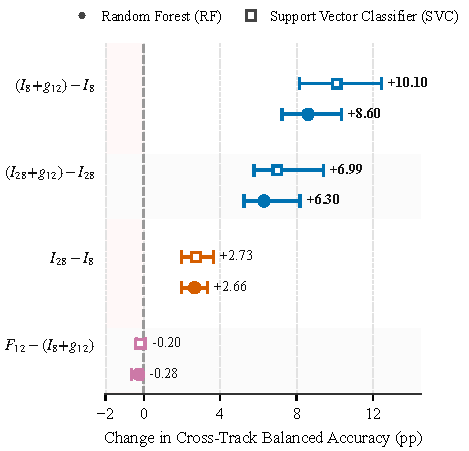
\includegraphics[width=0.48\textwidth]{fig14_coherence_ablation.pdf}
\caption{Nested representation contrasts in cross-track balanced accuracy with 95\% joint block bootstrap intervals. The comparisons separate added intensity features, raw coherence, and three derived coherence transformations.}
\label{fig:coherence_ablation}
\end{figure}

\subsection{Transfer Across Tracks}
\label{sec:matrix}
\label{sec:paired}
\label{sec:transfergap}
Coherence improves all twelve directional cross-track transfers for both learners (Supplementary Table~\ref{supp-tab:transfer_matrix}; Fig.~\ref{fig:transfer_matrix}). RF increments range from $+4.7$ to $+7.4\pp$, and SVC increments range from $+6.0$ to $+8.2\pp$. Baseline accuracy depends strongly on the ordered track pair: RF ranges from $60.9\%$ for T139$\to$T37 to $70.8\%$ for T37$\to$T15, while SVC ranges from $59.7\%$ to $70.9\%$. The largest RF increment occurs for T139$\to$T37.



\begin{figure*}[!t]
\centering
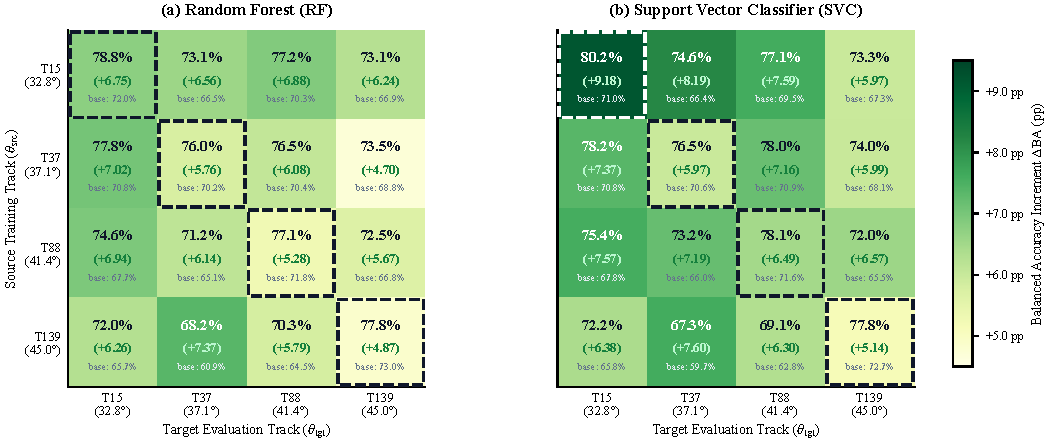
\includegraphics[width=0.94\textwidth]{fig5_transfer_matrix.pdf}
\caption{Balanced accuracy for all source--target track pairs under the 400\,m-buffered protocol: (a) RF and (b) SVC. Cells report baseline and augmented accuracy and their paired difference. Dashed outlines identify in-track evaluations.}
\label{fig:transfer_matrix}
\end{figure*}

In-track gains are close to cross-track gains: $+5.66$ versus $+6.30\pp$ for RF and $+6.69$ versus $+6.99\pp$ for SVC. The paired difference $\Delta_{\mathrm{cross}}-\Delta_{\mathrm{in}}$ is $+0.64\pp$ $[+0.07,+1.16]$ in balanced accuracy and $+0.26\pp$ $[-0.05,+0.54]$ in overall accuracy for RF. For SVC, the corresponding values are $+0.30\pp$ $[-0.01,+0.59]$ and $+0.19\pp$ $[-0.17,+0.62]$. Most of the coherence increment is shared by in-track and cross-track classification.

The directional transfer gap decreases from $4.76$ to $4.12\pp$ in RF balanced accuracy and from $4.74$ to $4.44\pp$ in SVC balanced accuracy (Supplementary Fig.~\ref{supp-fig:transfer_gap}). Overall-accuracy gaps decrease from $3.62$ to $3.35\pp$ and from $3.31$ to $3.12\pp$. These reductions equal the paired differences above; only the RF balanced-accuracy interval excludes zero.

Across distinct tracks, incidence-angle separation on $\Omega$ ranges from $3.62^\circ$ for T88$\leftrightarrow$T139 to $12.21^\circ$ for T15$\leftrightarrow$T139. The per-pair coherence increment has no monotone relationship with this separation. Regression summaries over all sixteen pairs, including the in-track anchors, give baseline and augmented slopes of $-0.41$ and $-0.34\pp/^\circ$ for RF and $-0.39$ and $-0.39\pp/^\circ$ for SVC (Supplementary Fig.~\ref{supp-fig:angular_disparity}).





\subsection{Class-Level Discrimination and Spatial Structure}
\label{sec:perclass}
\label{sec:confusion}
Built-up recall accounts for $74.5\%$ of the RF balanced-accuracy increment and $75.5\%$ of the SVC increment (Fig.~\ref{fig:class_decomposition}). Recall rises from $67.22\%$ to $90.71\%$ for RF and from $66.63\%$ to $93.01\%$ for SVC. Forest recall rises from $76.15\%$ to $81.13\%$ and from $78.30\%$ to $82.92\%$. Grassland changes by $+0.48$ and $-0.04\pp$, and cropland by $+1.24$ and $+1.18\pp$.

Equal class weighting assigns built-up gains contributions of $+4.70\pp$ and $+5.28\pp$ to balanced accuracy. Built-up occupies $1.72\%$ of the evaluation sample (165 unique pixels), so its RF contribution to overall accuracy is $+0.40\pp$. This sample-prevalence weighting explains the difference between the balanced-accuracy and overall-accuracy increments.

\begin{figure*}[!t]
\centering
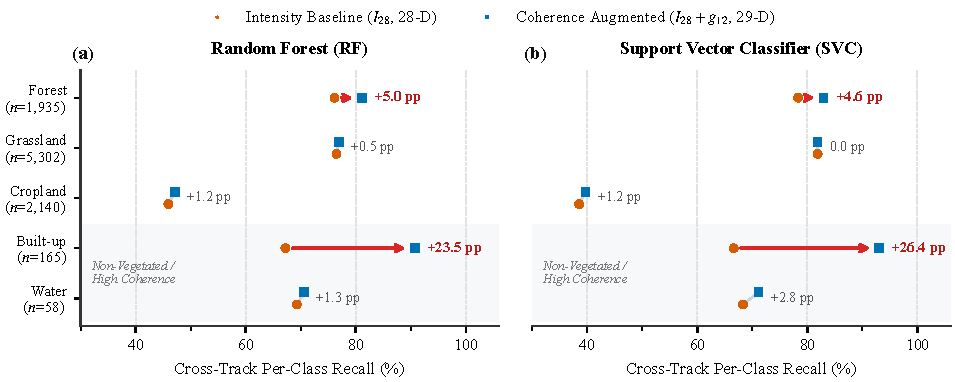
\includegraphics[width=0.94\textwidth]{fig6_class_decomposition.pdf}
\caption{Per-class cross-track recall for RF and SVC, pooled over twelve track pairs and three seeds. Orange circles denote $I_{28}$; blue squares denote $I_{28}+g_{12}$. Connectors show recall changes, with unique pixel counts below class names. Built-up and forest contribute the largest gains.}
\label{fig:class_decomposition}
\end{figure*}

The class signatures show a strong coherence contrast between built-up and vegetation on consensus support $C_2$ (Fig.~\ref{fig:coherence_distributions}). Across tracks, built-up median $g_{12}$ is $0.83$--$0.88$, with median two-date mean VV between $-7.8$--$-7.0$\,dB. Forest has median coherence $0.25$--$0.28$ and median VV between $-9.6$--$-8.7$\,dB. Grassland has median coherence $0.28$--$0.36$ and median VV between $-13.4$--$-12.4$\,dB. Open-water median VV is at most $-19.7$\,dB on every track. The built-up--forest median coherence separation ranges from $0.58$ to $0.62$ across the four viewing configurations.

\begin{figure*}[!t]
\centering
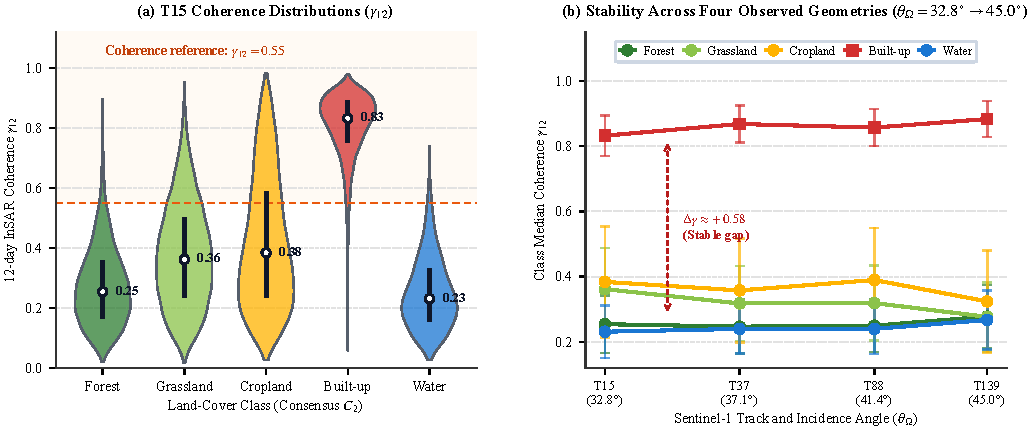
\includegraphics[width=0.98\textwidth]{fig7_coherence_distributions.pdf}
\caption{Class-specific 12-day coherence on consensus support $C_2$: (a) T15 distributions and (b) class medians across the four tracks. Violin densities use at most 10,000 pixels per class; medians and quartiles use all available class pixels. Error bars in (b) show half the interquartile range on either side of the median. On T15, built-up has median coherence $0.83$ and interquartile range $[0.76,0.88]$; its median separation from forest is $0.58$. Track incidence angles span approximately $32.8^\circ$--$45.0^\circ$.}
\label{fig:coherence_distributions}
\end{figure*}

The largest confusion change is the built-up/forest exchange (Table~\ref{tab:confusion}). RF assigns $17.5\%$ of built-up pixels to forest under $I_{28}$ and $0.8\%$ after adding coherence. The reciprocal error decreases from $6.9\%$ to $1.3\%$. SVC shows the same confusion pattern. Cropland remains strongly confused with grassland: the baseline assigns $45.1\%$ of cropland pixels to grassland, and cropland recall changes from $46.0\%$ to $47.2\%$ after augmentation.

\begin{table}[!t]
\caption{Pooled Cross-Track Confusion Matrix for the Random Forest Under the Buffered Protocol, Row-Normalised (\%).
Each Cell Reads $I_{28} \rightarrow I_{28}+g_{12}$; Cells Changing by Less Than $1\pp$ Are Shown Once.}
\label{tab:confusion}
\centering
\scriptsize
\setlength{\tabcolsep}{2.5pt}
\begin{tabular}{lccccc}
\toprule
True $\backslash$ Pred. & Forest & Grass. & Crop. & Urban & Water \\
\midrule
Forest & \textbf{76.2$\to$81.1} & 13.2 & 3.8 & 6.9$\to$1.3 & 0.0 \\
Grassland & 5.3 & \textbf{76.5} & 16.7 & 1.5 & 0.0 \\
Cropland & 5.8 & 45.1 & \textbf{46.0$\to$47.2} & 3.0$\to$1.5 & 0.2 \\
Urban & 17.5$\to$0.8 & 7.7$\to$3.4 & 7.6$\to$5.1 & \textbf{67.2$\to$90.7} & 0.0 \\
Water & 0.7 & 10.1$\to$11.2 & 19.6$\to$16.9 & 0.3 & \textbf{69.3$\to$70.6} \\
\midrule
Support & 69{,}660 & 190{,}872 & 77{,}040 & 5{,}940 & 2{,}088 \\
\bottomrule
\end{tabular}
\\[2pt]
\parbox{\columnwidth}{\footnotesize Support is the cumulative number of predictions over 12 ordered track pairs and 3 seeds ($36\times$ the underlying unique evaluation pixels: 1{,}935 / 5{,}302 / 2{,}140 / 165 / 58). The block bootstrap resamples entire geographic blocks with replacement, carrying all 36 repetitions together, so this pooled support does not inflate the effective sample size.}
\end{table}

Spatial maps show how these class-level changes alter settlement delineation. In the illustrated Wierden/Almelo region spanning evaluation blocks 205 and 206, coherence corrects 176 of 192 false forest predictions over settlement pixels, a $91.7\%$ reduction (Fig.~\ref{fig:spatial_maps}). In the suburban fringe of Block~803, the illustrated T15$\to$T37 transfer gains $24.2\pp$ in local built-up recall (Supplementary Fig.~\ref{supp-fig:multilandscape_maps}). The rural landscape in Block~603 gains $37.5\pp$, with farmsteads and infrastructure recovered in the augmented map. These examples display the spatial pattern of the pooled confusion changes.

\begin{figure*}[!t]
\centering
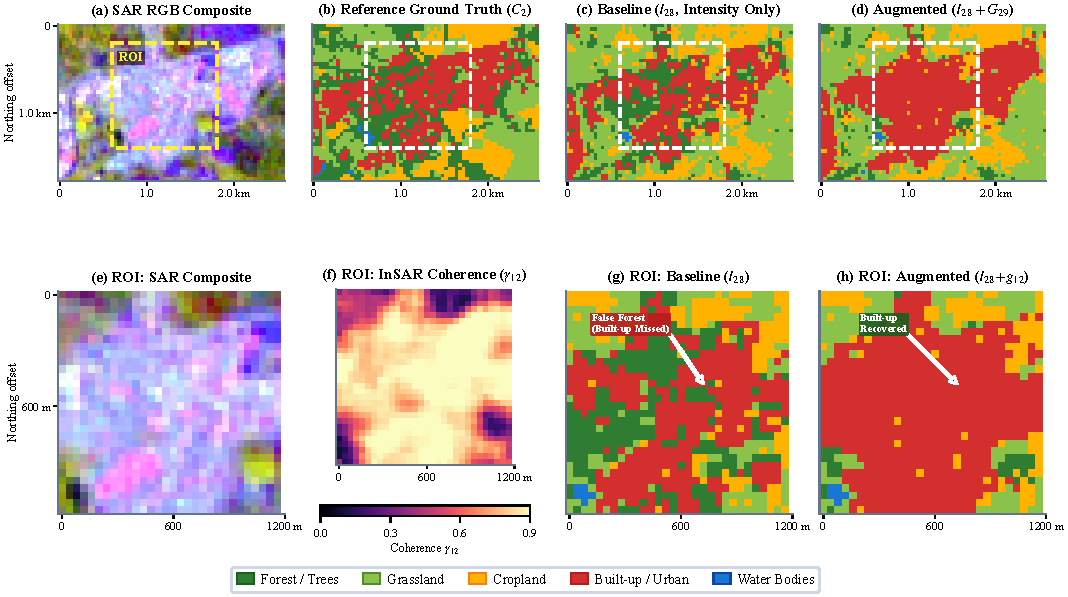
\includegraphics[width=0.98\textwidth]{fig8_spatial_classification.pdf}
\caption{Spatial classification maps and pixel-level error resolution over real Sentinel-1 SAR observations in evaluation blocks 205 and 206 (Wierden/Almelo, Overijssel, Netherlands; $1.8 \times 2.6$\,km macro domain, $1.2 \times 1.2$\,km inset ROI). (a) False-color SAR observation ($\gamma^0_{\mathrm{VV}}$, $\gamma^0_{\mathrm{VH}}$, $\gamma_{12}$). (b) Harmonized consensus ground truth ($C_2$). (c) Baseline $I_{28}$ predictions exhibiting widespread false forest confusion over urban structures. (d) Coherence-augmented $I_{28}{+}g_{12}$ predictions restoring urban settlements. (e--h) Zoomed ROI details showing: (e) high-resolution SAR composite, (f) 12-day InSAR coherence heatmap ($\gamma_{12}$), (g) baseline error map highlighting 192 false forest pixels, and (h) coherence recovery map correcting 176 pixels ($91.7\%$ confusion reduction).}
\label{fig:spatial_maps}
\end{figure*}



\label{sec:labelaudit}
The 165 built-up evaluation pixels occupy 16 connected objects in eight of the twelve evaluation blocks. One block contains $38.8\%$ of these pixels; the largest object contains $53.3\%$, and the five largest contain $88.5\%$ (Supplementary Fig.~\ref{supp-fig:labelaudit}). At 40\,m posting, $55.8\%$ lie within 40\,m of a class boundary and $78.8\%$ within 80\,m. Fully built-up $3\times3$ and $5\times5$ neighbourhoods occur for $12.7\%$ and $3.0\%$ of the sampled pixels. The minimum-mapping-unit filter removes $16.4\%$ of built-up label pixels, compared with $1.4\%$ of grassland pixels.



\subsection{Robustness to Support and Reference Labels}
\label{sec:label_independence}
North, south, and east directional holdouts retain positive coherence increments with a 5\,km excluded buffer. RF balanced-accuracy increments are $5.83$, $7.75$, and $7.27\pp$, respectively; SVC increments are $8.52$, $8.46$, and $8.07\pp$. These separate spatial partitions extend the comparison to contiguous held-out regions.

Coherence gains remain positive on interior built-up pixels and across object exclusions (Table~\ref{tab:builtup_audit}). Restricting evaluation to the 50 pixels at least 80\,m from a class boundary gives built-up recall increments of $+15.33\pp$ for RF and $+17.44\pp$ for SVC. On the 21 pixels with a fully built-up $3\times3$ neighbourhood, the increments are $+11.90$ and $+15.08\pp$. Both restrictions reduce the increment relative to the full built-up sample.

Resampling the 16 connected objects while holding the other class recalls fixed gives five-class increments of $+6.30\pp$ $[5.56,8.32]$ and $+6.99\pp$ $[6.01,9.70]$. Leaving each object out in turn produces ranges of $+6.02$ to $+7.42\pp$ for RF and $+6.61$ to $+8.46\pp$ for SVC. Removing the largest sampled object increases the increments to $+7.42$ and $+8.46\pp$.

Excluding built-up from the metric gives four-class balanced-accuracy increments of $+2.01\pp$ $[1.50,2.63]$ for RF and $+2.14\pp$ $[1.62,2.73]$ for SVC, with forest providing the largest remaining recall gain. At block level, the five-class increment is positive in all twelve blocks for both learners (two-sided sign test, $p=0.0005$). RF block increments range from $+0.97$ to $+14.95\pp$, with mean $+5.81\pp$; SVC increments range from $+1.07$ to $+17.29\pp$, with mean $+6.27\pp$ (Supplementary Fig.~\ref{supp-fig:spatial_sign_test}).

\begin{table}[!t]
\caption{Audit of the 165 Built-Up Evaluation Pixels. Recall Values Are Cross-Track, Pooled Over
Twelve Ordered Track Pairs and Three Seeds.}
\label{tab:labelaudit}\label{tab:builtup_audit}
\centering
\scriptsize
\setlength{\tabcolsep}{3pt}
\begin{tabular}{lcccc}
\toprule
& \multicolumn{2}{c}{Random forest} & \multicolumn{2}{c}{SVC} \\
\cmidrule(lr){2-3}\cmidrule(lr){4-5}
Subset / test & $I_{28}$ & $I_{28}{+}g_{12}$ & $I_{28}$ & $I_{28}{+}g_{12}$ \\
\midrule
\multicolumn{5}{l}{\emph{Built-up recall (\%)}} \\
All 165 pixels                          & 67.22 & \textbf{90.71} & 66.63 & \textbf{93.01} \\
$\geq 80$\,m from a class boundary (50) & 80.33 & 95.67 & 79.11 & 96.56 \\
Fully built-up $3\times3$ (21)          & 84.79 & 96.69 & 84.13 & 99.21 \\
\midrule
\multicolumn{5}{l}{\emph{Five-class $\Delta\text{BA}$ (pp) under alternative treatments}} \\
Block bootstrap    & \multicolumn{2}{c}{$+6.30$ $[5.25, 8.19]$} & \multicolumn{2}{c}{$+6.99$ $[5.78, 9.39]$} \\
Object-clustered bootstrap   & \multicolumn{2}{c}{$+6.30$ $[5.56, 8.32]$} & \multicolumn{2}{c}{$+6.99$ $[6.01, 9.70]$} \\
Leave-one-object-out range   & \multicolumn{2}{c}{$+6.02$ to $+7.42$}     & \multicolumn{2}{c}{$+6.61$ to $+8.46$} \\
Largest object (88 px) removed & \multicolumn{2}{c}{$+7.42$}              & \multicolumn{2}{c}{$+8.46$} \\
Built-up class removed (4-class BA) & \multicolumn{2}{c}{$+2.01$ $[1.50, 2.63]$} & \multicolumn{2}{c}{$+2.14$ $[1.62, 2.73]$} \\
12-block sign test ($k/12 > 0$)     & \multicolumn{2}{c}{12/12 ($p = 0.0005$)} & \multicolumn{2}{c}{12/12 ($p = 0.0005$)} \\
\bottomrule
\end{tabular}
\\[2pt]
\parbox{\columnwidth}{\footnotesize The object-clustered bootstrap resamples the 16 connected built-up objects with replacement and varies only the built-up recall term, the other four class recalls being held at their point estimates; the block bootstrap varies all five class recalls. For the 4-class balanced accuracy (built-up excluded), 95\% confidence intervals are derived from 20{,}000 paired block bootstrap draws conditioned on complete 4-class presence (19{,}306 valid replicates, 3.47\% whole-class water dropout excluded, identical to the 5-class protocol).}
\end{table}



The label-source analysis also gives positive increments for every training/evaluation label combination (Table~\ref{tab:label_independence_controls}). Under the buffered label-sensitivity protocol, WC$\to$WC yields $+3.64\pp$ for RF and $+6.68\pp$ for SVC on common valid support $U_2$. CLC$\to$CLC yields $+6.53$ and $+8.46\pp$. The cross-product evaluations give $+5.54$ and $+8.76\pp$ for WC$\to$CLC, and $+4.14$ and $+5.69\pp$ for CLC$\to$WC.

On consensus support $C_2$, consensus-trained models yield $+7.02$ and $+7.60\pp$, while WC-trained and WC-evaluated models yield $+6.96$ and $+11.07\pp$. The analysis uses $U_2=600{,}317$ valid pixels on $\Omega=608{,}825$ and $C_2=287{,}013$ consensus pixels. This analysis samples up to 800 evaluation pixels per block on $U_2$, then restricts that sample to $C_2$ for consensus evaluations. Each model uses 20{,}000 training pixels, a 400\,m exclusion from the $U_2$ evaluation sample, and the selected R1 hyperparameters. Its consensus evaluation support therefore differs from the primary benchmark. Positive increments are observed with both reference products and their cross-product evaluations.

\begin{table}[!t]
\caption{Cross-Track Balanced Accuracy Increment ($\Delta\text{BA}$, pp) Across Reference Label Products and Support Sets With 400\,m Training--Evaluation Exclusion.}
\label{tab:label_independence_controls}
\centering
\scriptsize
\setlength{\tabcolsep}{1.8pt}
\begin{tabular}{lllcc}
\toprule
Train Label & Eval Label & Support & RF $\Delta\text{BA}$ & SVC $\Delta\text{BA}$ \\
\midrule
WorldCover (WC) & WorldCover (WC) & Common ($U_2$) & $+3.64$ & $+6.68$ \\
WorldCover (WC) & CORINE (CLC)    & Common ($U_2$) & $+5.54$ & $+8.76$ \\
CORINE (CLC)    & WorldCover (WC) & Common ($U_2$) & $+4.14$ & $+5.69$ \\
CORINE (CLC)    & CORINE (CLC)    & Common ($U_2$) & $+6.53$ & $+8.46$ \\
Consensus ($C_2$) & Consensus ($C_2$) & Consensus ($C_2$) & $+7.02$ & $+7.60$ \\
WorldCover (WC) & WorldCover (WC) & Consensus ($C_2$) & $+6.96$ & $+11.07$ \\
\bottomrule
\end{tabular}
\\[2pt]
\parbox{\columnwidth}{\footnotesize Mean paired increments across twelve ordered cross-track pairs and three seeds. Models use frozen R1 hyperparameters and 20{,}000 training pixels. Consensus evaluations use the agreeing subset of the sampled $U_2$ evaluation pixels.}
\end{table}

\subsection{Temporal Replication}
\label{sec:temporal_validation}
The coherence increment remains positive in balanced accuracy for the October 2024 acquisition window (Table~\ref{tab:temporal_validation}). Across the same four tracks and twelve evaluation blocks, RF balanced accuracy increases from $62.91\%$ to $67.93\%$ ($+5.03\pp$), and SVC increases from $63.01\%$ to $68.24\%$ ($+5.23\pp$). The corresponding 95\% bias-corrected and accelerated block bootstrap intervals are $[3.33,7.08]$ and $[3.36,7.27]\pp$.

Autumn overall-accuracy increments are $+0.62\pp$ for RF and $-0.01\pp$ for SVC, with percentile intervals $[-0.36,1.74]$ and $[-0.68,0.79]\pp$. Built-up recall increases from $75.00\%$ to $96.08\%$ for RF and from $73.82\%$ to $97.04\%$ for SVC, giving gains of $+21.08$ and $+23.22\pp$. Forest recall gains are $+4.10$ and $+1.05\pp$.

\begin{table*}[!t]
\caption{Temporal Replication Benchmark: Spring 2024 vs. Autumn 2024 Cross-Track Evaluation Under Observation Budget Parity ($N=2$)}
\label{tab:temporal_validation}
\centering
\scriptsize
\setlength{\tabcolsep}{6pt}
\begin{tabular}{lcccc}
\toprule
& \multicolumn{2}{c}{Spring 2024} & \multicolumn{2}{c}{Autumn 2024 (Temporal Replication)} \\
\cmidrule(lr){2-3}\cmidrule(lr){4-5}
Evaluation Metric / Diagnostic Quantity & Random Forest & SVC & Random Forest & SVC \\
\midrule
Five-Class Balanced Accuracy Increment ($\Delta\text{BA}$, pp) & $+6.30$ & $+6.99$ & $+5.03$ & $+5.23$ \\
\quad 95\% Joint Block Bootstrap Interval                      & $[5.25, 8.19]$ & $[5.78, 9.39]$ & $[3.33, 7.08]$ & $[3.36, 7.27]$ \\
Sample Overall Accuracy Increment ($\Delta\text{OA}$, pp)& $+1.95$ & $+1.64$ & $+0.62$ & $-0.01$ \\
\quad 95\% Joint Block Bootstrap Interval                      & $[1.32, 2.65]$ & $[0.91, 2.47]$ & $[-0.36, 1.74]$ & $[-0.68, 0.79]$ \\
Built-Up Class Recall Gain ($\Delta\text{Recall}$, pp)           & $+23.48$ & $+26.38$ & $+21.08$ & $+23.22$ \\
\quad Absolute Recall Shift (Baseline $\to$ Augmented)         & $67.2\% \to 90.7\%$ & $66.6\% \to 93.0\%$ & $75.0\% \to 96.1\%$ & $73.8\% \to 97.0\%$ \\
Four-Class Balanced Accuracy Increment (Without Built-Up, pp)             & $+2.01$ & $+2.14$ & $+1.01$ & $+0.74$ \\
12-Block Spatial Consistency (Sign Test $k/12 > 0$)             & 12/12 ($p = 0.0005$) & 12/12 ($p = 0.0005$) & 9/12 ($p = 0.146$) & 10/12 ($p = 0.0386$) \\
\bottomrule
\end{tabular}
\\[2pt]
\parbox{\textwidth}{\footnotesize All metrics evaluated across all 12 ordered cross-track pairs ($n=12$) on the identical 12 evaluation blocks and $C_2$ consensus ground-truth support under strict observation budget parity ($N=2$). Spring intervals use the joint block percentile bootstrap. Autumn balanced-accuracy intervals use the bias-corrected and accelerated bootstrap; autumn overall-accuracy intervals use the percentile bootstrap (20{,}000 draws).}
\end{table*}

Removing built-up leaves four-class balanced-accuracy increments of $+1.01\pp$ for RF and $+0.74\pp$ for SVC, compared with $+2.01$ and $+2.14\pp$ in spring. Positive block increments occur in 9 of 12 autumn blocks for RF ($p=0.146$) and 10 of 12 for SVC ($p=0.0386$). The autumn results retain the concentration of gains in built-up classification, with smaller five-class increments and weaker spatial consistency than in spring.

\section{Discussion}
\label{sec:mech}

Coherence is most useful when the mapping task requires separating surfaces with similar backscatter but different temporal stability. Bright returns from buildings and forest can overlap in intensity, while persistent structures and changing canopy scatterers generate distinct repeat-pass coherence distributions~\cite{Sica2019,Aghababaei2026}. This distinction gives the observable a clear role in mixed rural landscapes, where small settlements are embedded in vegetation. The class distributions and error maps connect that scattering interpretation to the recovery of built-up land cover. For deployment, the relevant question is therefore whether temporal stability separates the classes that matter to the application. A landscape containing many rigid structures next to forest presents a different classification problem from one dominated by agricultural classes with similar 12-day decorrelation.

Recent interferometric studies help explain why the coherence contrast is informative. Forest scattering models link repeat-pass coherence to canopy and ground contributions~\cite{Aghababaei2026}. Crop growth and soil-moisture changes alter interferometric observations through vegetation development and dielectric properties~\cite{Yuan2024,Ao2025}, while random motion produces temporal decorrelation~\cite{Chen2026}. The resulting sensitivity to surface change also underlies the amplitude--coherence inputs used by DANI-NET for change detection~\cite{Costa2025}. Here, that temporal sensitivity supplies a class-discriminating feature at a single repeat interval.

The evaluation objective determines how that class separation translates into practical value. Sample overall accuracy weights each class-recall change by its prevalence in the evaluation sample. Balanced accuracy assigns every class equal weight. A coherence feature can consequently contribute strongly to settlement detection while producing a smaller change in scene-wide accuracy. For an application that must retain small settlements, built-up recall and its spatial support are directly relevant alongside balanced accuracy. For land-cover inventories, sample overall accuracy describes the aggregate outcome on the evaluated support. Reporting both connects the same classifier to these different objectives. The spring and autumn evaluations further motivate tracking class-level performance across acquisition windows: the mapping benefit depends on the distribution of errors among classes as well as the separability of built-up land cover.

At a two-acquisition budget, coherence extracts temporal information from the complex image pair already used by the intensity representation. The compact $I_8{+}g_{12}$ representation offers a practical starting point for deployment, retaining the observed discrimination with few feature channels. The ablation supports using the raw scalar directly; spatial coherence derivatives add processing steps without improving the evaluated classifiers. Acquiring and processing a suitable interferometric pair is thus the central operational requirement. Once coherence is available, deployment can begin with the compact representation and compare its performance with the richer intensity features on the intended source--target track pair. Pair-specific validation remains useful because acquisition configuration determines the classifier's operating accuracy. The broader methodological contribution is a comparison in which additional feature information is evaluated at a fixed observation budget. Applying this same design to other budgets would make acquisition planning and representation choice part of a common quantitative assessment.

Coherence estimation provides a concrete avenue for extending this representation. Recent methods select similarly decorrelated neighborhoods~\cite{Yao2024}, reduce low-coherence estimation bias~\cite{LiangH2026}, and estimate interferometric parameters with self-supervised learning~\cite{Geara2025}. MTCSAR uses a coherence prior to guide multitemporal SAR denoising~\cite{LiuJ2025}. The observation model also matters: burst-mode phase separation~\cite{Pulella2024} and analyses of range misregistration~\cite{Yang2026} connect interferometric measurements to acquisition and processing geometry. An extension can compare these estimators at the same acquisition budget and measure the resulting change in class discrimination.

Acquisition planning can build on coherence proxies that describe baseline and seasonal variation~\cite{Xu2025}, while scatterer-specific stochastic models address time-varying interferometric observation quality~\cite{Brouwer2025}. For land-cover products, field-boundary mapping offers an object-level complement to pixel classification~\cite{Celik2026}. Spatial and temporal validation of vegetation estimates likewise connects representation choice to deployment conditions~\cite{WangX2025}. Together, these developments suggest a practical sequence: select the repeat-pass pair, estimate the additional observable, and evaluate its contribution on the spatial units relevant to the mapping product.

The present evidence concerns orbital and seasonal deployment within one region. Acquisition geometry and date vary together, so the class-separation result describes their combined operating conditions. The built-up sample contains 165 pixels from 16 objects, and the reference maps predate the SAR acquisitions; support and label-sensitivity diagnostics are provided in the supplement. Geographic replication with contemporaneous labels is the next test of the measured effect sizes.

\section{Conclusion}

A single 12-day interferometric coherence measurement adds substantial class-discriminating information to two-acquisition Sentinel-1 land-cover classification. Against a spatially tuned 28-D intensity baseline, it increased cross-track balanced accuracy by $6.30\pp$ for RF and $6.99\pp$ for SVC, with overall-accuracy gains of $1.95\pp$ and $1.64\pp$. The four-track comparison ties this improvement to stronger built-up/forest separation. Comparable in-track gains identify temporal stability as useful class information across deployment configurations. The compact nine-dimensional representation retains nearly all of the performance achieved by the larger augmented feature set, providing a simple implementation of this finding.

The study quantifies coherence's marginal value while holding the acquisition budget, training support, and model-selection procedure constant. Its representation ladder links feature choice to class-level error recovery, and the paired spatial evaluation measures the gain across ordered orbital transfers. Autumn replication retained balanced-accuracy gains of $5.03\pp$ and $5.23\pp$ for the two learners. Together, these experiments provide an empirical basis for including raw coherence in low-observation land-cover mapping and a reproducible framework for evaluating additional SAR observables against competitive intensity representations.


\begingroup\raggedright
\bibliographystyle{IEEEtran}
\bibliography{references}
\endgroup

\end{document}
